\documentclass[dvipdfmx,tikz]{standalone}
\usepackage{tikz,bm}
\usetikzlibrary{intersections,calc,arrows}
\begin{document}
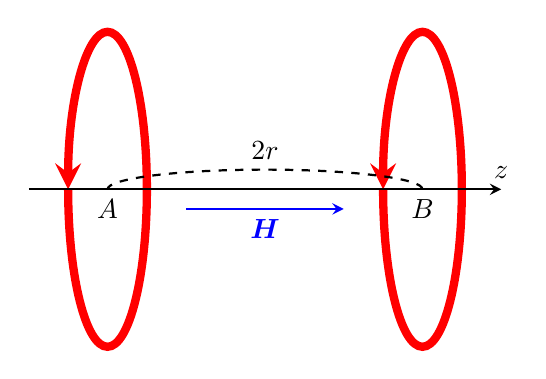
\begin{tikzpicture}
%\draw[help lines] (-3,-2) grid (3,2);
\draw[->,>=stealth,color = red,line width=3pt]
    (-2.5,0) arc [start angle=-180, end angle=180,x radius=0.5, y radius=2];
\draw[->,>=stealth,color = red,line width=3pt]
    (1.5,0) arc [start angle=-180, end angle=180,x radius=0.5, y radius=2];
\draw[->,>=stealth,thick] (-3,0) -- (3,0) node[above] {$z$};
\draw[>=stealth,thick,dashed]
    (2,0) arc [start angle=0, end angle=180,x radius=2, y radius=0.25]node[midway,above] {$2r$};
\node (A) at (-2,-0.25) {$A$}; 
\node (B) at (2,-0.25) {$B$};
\draw [->,>=stealth,color = blue,thick] (-1,-0.25) -- (1,-0.25) node[midway,below] {$\bm{H}$};
\end{tikzpicture}
\end{document}